\documentclass{article}
\usepackage{csquotes}
\usepackage[english]{babel}
\usepackage{amsmath}
\usepackage{graphicx}
\usepackage{hyperref}
\usepackage{multirow}
\usepackage{microtype}
\usepackage[backend=biber, sorting=none]{biblatex}
\usepackage{listings}
\lstset{breaklines=true,basicstyle=\footnotesize,language=Python}
\usepackage[normalem]{ulem}
\addbibresource{refs.bib}
\AtBeginBibliography{\raggedright}
%\usepackage{multicol}
\usepackage{emoji}

\title{ACARIS: Attempting to Improve Conversational AI and Human Social Skills using User Embeddings}
\author{Simon Slamka\\
\small\textbf{OngakkenAI}}
\date{June 21, 2023}

\begin{document}

\maketitle

\begin{abstract}
In this paper, we propose ACARIS, the Advanced Communication Augmentor and Relational Insights System, a system utilizing a novel method to analyze emotional state, intent, and interest of text communication parties. ACARIS is being built with the goal of improving social skills of humans, while also improving the performance of human-facing AI systems. We go over our initial approach, including the initialization of user embeddings from message features, concatenation of user embeddings with word embeddings, modifications of the DistilBERT architecture, and the training and evaluation processes. We also go over the results of our experiments. Presently, we are not able to achieve any statistically nor practically significant improvement over the current state-of-the-art. However, we actively continue to work on improving our approach by iterating over different architectures, hyperparameters, and user embedding forms. In addition, the work currently only handles sentiment analysis, as other tasks are still in heavy development. As such, the target variable of the model is a sentiment label, and as such, the model is a classifier.
\end{abstract}

\section{Introduction}
\subsection{Keywords}
ACARIS, Conversational AI, Social Skills, User Embeddings, BERT, DistilBERT, Sentiment Analysis, Intent Classification, Emotion Recognition, Interest Recognition

\subsection{Definitions}
\begin{itemize}
	\item \textbf{ACARIS} - the Advanced Communication Augmentor and Relational Insights System
	\item \textbf{NLP} - Natural Language Processing - a subfield of linguistics, computer science, and artificial intelligence concerned with the interactions between machines and human language, in particular how to program computers to process and analyze large amounts of natural language data
	\item \textbf{Deep learning} - a class of machine learning algorithms that uses multiple layers to progressively extract higher-level features from the raw input
	\item \textbf{Paired t-test} - a statistical procedure used to determine whether the mean difference between two sets of observations is zero
	\item \textbf{Shapiro-Wilk test} - a test of normality in frequentist statistics
	\item \textbf{p-value} - the probability of obtaining results as extreme as the observed results of a statistical hypothesis test, assuming that the null hypothesis is correct
	\item \textbf{Wilcoxon signed-rank test} - a non-parametric statistical hypothesis test used when comparing two related samples, matched samples, or repeated measurements on a single sample to assess whether their population mean ranks differ
	\item \textbf{Decision boundary} - a hypersurface that partitions the underlying vector space into two sets, one for each class
	\item \textbf{model accuracy score} - the fraction of predictions a model got right
	\item \textbf{model precision score} - the fraction of positive predictions a model got right
	\item \textbf{model recall score} - the fraction of positive cases a model got right
	\item \textbf{model support score} - the number of occurrences of each class in y\_true
	\item \textbf{model F1 score} - the harmonic mean of precision and recall
	\item \textbf{ROC curve} - the Receiver Operating Characteristic curve
	\item \textbf{model AUC score} - the area under the ROC curve - a plot of the true positive rate against the false positive rate
	\item \textbf{SVM} - Support Vector Machine - a supervised machine learning model that uses classification algorithms for two-group classification problems
	\item \textbf{DT} - Decision Tree - a decision support tool that uses a tree-like model of decisions and their possible consequences
	\item \textbf{LogReg} - Logistic Regression - a statistical model that in its basic form uses a logistic function to model a binary dependent variable, although many more complex extensions exist
	\item \textbf{RF} - Random Forest - an ensemble learning method for classification, regression and other tasks that operate by constructing a multitude of decision trees at training time and outputting the class that is the mode of the classes (classification) or mean prediction (regression) of the individual trees
	\item \textbf{TF-IDF} - Term Frequency - Inverse Document Frequency - a numerical statistic that is intended to reflect how important a word is to a document in a collection or corpus, calculated as the product of its term frequency and its inverse document frequency. Has no sense of word order
	\item \textbf{the Transformer} - a deep learning architecture introduced in 2017, used primarily in the field of NLP\cite{vaswani2017attention}
	\item \textbf{BERT} - Bidirectional Encoder Representations from Transformers - a transformer-based machine learning model for natural language processing pre-training developed by Google\cite{devlin2019bert}
	\item \emoji{hugging-face} - Hugging Face - a company that develops and maintains open-source libraries for natural language processing
	\item \textbf{DistilBERT} - DistilBERT is a smaller, faster, cheaper version of BERT developed by \emoji{hugging-face}\cite{sanh2020distilbert}
	\item \textbf{Vector} - a quantity that has both magnitude and direction
	\item \textbf{Vector space} - a collection of vectors, which may be added together and multiplied ("scaled") by numbers, called scalars
	\item \textbf{Embedding space} - a vector space with a coordinate for each word in the vocabulary, such that words that share common contexts in the corpus are located close to one another in the space
	\item \textbf{Word embedding} - A vector representation of a word's meaning
	\item \textbf{User embedding} - A vector representation of a user's personality, emotional state, intent, and interest
	\item \textbf{FFNN} - Feed-Forward Neural Network - a neural network where connections between units do not form a cycle
	\item \textbf{ReLU} - Rectified Linear Unit - an activation function that returns the input value if it is positive, otherwise it returns zero
	\item \textbf{Loss} - a number indicating how bad the model's prediction was on a single example
	\item \textbf{Cross-entropy loss} - negative logarithmic likelihood loss - a loss function used for classification problems
	\item \textbf{Adam} - an optimization algorithm that can be used instead of the classical stochastic gradient descent procedure to update network weights
\end{itemize}
\subsection{Motivation}
I've always had an issue with interpersonal relationships. I could never fully understand the way people work on a social level. I understand the technical and biological fundamentals, and superficially, how the mind works, but not how all this becomes so much more complex when actually talking and dealing with people. Sometimes, I feel that another person and I broadcast on different frequencies, because we are unable to either understand one another or maintain a (romantic) relationship for an extended period of time. I have tried for many years to find a technical solution to this problem, but only after coming to Denmark, I acquired the core knowledge to try and accomplish this ambitious goal by really getting into it and self-studying as much as I could.\\
I firmly believe that all things in nature are governed by rules and these rules can be observed, measured, and then, based on that data, predicted. This includes human behavior and emotions. We’re nothing more than complex electrobiochemical machines driven by electrical impulses and hormones. Apart from that, even if we don’t understand our own minds yet, we still have many, many years of knowledge about how human personalities work and how we make decisions based on what happens to or around us. On a fundamental level, this doesn’t change. Sure, they say that we’re all different. However, the core remains. We all share many attributes that make us human. I believe that we, given enough data, can use these attributes to predict human behavior, reactions, emotional state, and intent.

\subsection{Hypotheses}
\subsubsection{$H_1$}
Given enough conversational data per person, human behavior (personality, emotional state, intent, and interest rate) in text communication can be predicted with a high level of confidence ($>80\%$) due to the fact that humans are, on a fundamental level, very similar to one another.

Additionally, we posit that person-specific performance improvements can be achieved by individualizing predictions by using a unique vector representation of a person's personality, emotional state, intent, and interest rate, which we call a user embedding. The postulate stems in the core concept of neural networks being universal function approximators. Therefore, in theory, a neural network should be able to learn to associate a user embedding with a person's behavior in text communication and use that information to improve its predictions.

\subsubsection{$H_0$}
The performance of a human behavior analysis model trained using a user embedding is not significantly different from the performance of a human behavior analysis model trained purely with input sequences as the model's input.

\subsubsection{Statistical significance}
To test the statistical significance between the ACARIS and the baseline models, we use paired t-tests or, if the metrics are not normally distributed, Wilcoxon signed-rank tests. A p-value of $<0.05$ is considered statistically significant.

\subsubsection{Practical significance}
To test the practical significance between the ACARIS and the baseline models, we define a decision boundary of practical significance as a model performance improvement of the ACARIS model over the baseline model of $>=5\%$ across all calculated model performance metrics, simultaneously. Namely, these are accuracy, precision, recall, F1, and AUC.

%\begin{multicols}{2}
\subsection{Premise}
Interpersonal communication has always been an integral part of human lives and is critical from the moment we're born. With the rise of the Internet and, subsequently, social media and other forms of online text communication, the manner in which we talk has changed dramatically. This has led to a drop in social skills in humans, particularly those of the last generation. ACARIS attempts to adjust for this by providing a way to analyze the emotional state, intent, and interest of text communication parties, providing them with a way to improve their social skills, while also improving the performance of conversational AI systems, which are becoming increasingly prevalent in our society, and their ability to understand human emotions, intent, and interest is becoming more and more important, especially in AI systems that directly interact with humans, such as digital assistants, chatbots, and others.

\subsection{Literature Review and Related Work}
\subsubsection{Studied Literature}
\begin{itemize}
	\item \textbf{Machine Learning with PyTorch and Scikit-Learn}\cite{raschka2022machine} by Yuxi Liu, Vahid Mirjalili, Sebastian Raschka
	\item \textbf{Hands-on Machine Learning with Scikit-Learn, Keras, and TensorFlow}\cite{geron2022hands} by Aurélien Géron
	\item \textbf{Transformers for Natural Language Processing}\cite{rothman2022transformers} by Denis Rothman, Antonio Gulli
	\item \textbf{Transformers for Machine Learning: A Deep Dive}\cite{kamath2022transformers} by Uday Kamath, Kenneth L. Graham, Wael Emara
\end{itemize}
\subsubsection{Related Work}
\begin{itemize}
	\item \textbf{Human-AI Collaboration Enables More Empathic Conversations in Text-based Peer-to-Peer Mental Health Support}\cite{sharma2022humanai}
	\item \textbf{Context Matters: Recovering Human Semantic Structure from Machine Learning Analysis of Large-Scale Text Corpora}\cite{https://doi.org/10.1111/cogs.13085}
\end{itemize}

\subsection{Initial attempts}
Our initial attempts of implementing ACARIS included the use of SVMs, DTs, LogReg, and RFs, each paired with TF-IDF in the preprocessing stage. None of these methods have proven to be accurate enough (barely reaching 50\% accuracy) for large amounts of complex language, especially casual language that often includes slang, sarcasm, emoji, and similar elements. The primary issue was the lack of these methods' ability to capture semantic and contextual aspects of our dataset. SVMs, DTs, LogReg, and RFs weren't built specifically for sequential data. For sequential data, RNNs and CNNs were classically used. However, due to the long-range dependency problem of RNNs, we made the decision to not use them, as we believed that they would not be able to capture the long-range dependencies in our dataset. Additionally, we weren't able to guarantee that during inference, there would be no long-range dependencies.
Another issue was TF-IDF's lack of word order and semantic meaning understanding. Knowing that the Transformer\cite{vaswani2017attention} architecture is capable of capturing these aspects due to its positional encodings and self-attention mechanism, we decided to use it as the basis for ACARIS.

\subsection{Short intro on Transformers}
The Transformer is a deep learning model architecture proposed in 2017 by a team of Google Brain/Google Research researchers. It is mainly used in NLP, but it has also found its way into numerous vision projects (Latent Diffusion\cite{rombach2021highresolution}/Stable Diffusion/LLaVA\cite{liu2023visual}, to name a few). The architecture aims to replace RNNs by using attention mechanisms (self-attention, in particular) and positional encodings to model long-range dependencies in sequential data.

\section{Methodology}
In this section, we provide a detailed description of our approach, including the computation of user embeddings, concatenation with word embeddings, modifications to the model architecture, and the training and evaluation processes.

\subsection{Dataset}
To build our dataset, we collected ~65 thousand messages from our Discord server, classified them into 3 classes (pos, neg, neu), and augmented the dataset with the following additional datasets: GoEmotions\cite{demszky2020goemotions} dataset, which contains 58 thousand messages classified into 27 classes. We squashed the 27 classes into 3 classes (pos, neg, neu); Twitter Sentiment and Emotion Analysis\cite{Cop_2021} containing 6032 rows of tweets labeled positive, negative, and neutral; Twitter-Sentiment Data\cite{Kumar_2022} containing 1975 rows of tweets labeled into the same three classes. To minimize error caused by input data, we removed all users with less than 25 messages, URLs, markdown code blocks, Discord mentions and custom emoji, and attachments. We also removed all messages shorter than 25 characters. The resulting dataset was split into 75\% training, 17\% validation, and 8\% test sets, and contains 24769, 5504, and 2753 rows, respectively (filtered). The discrepancy most likely stems in our splitting algorithm's static seed. The dataset is not publicly available at the moment due to the sensitive nature of the data.

\subsection{User Embeddings Initialization}
For each user $u$, we loop through all messages $m$ sent by $u$ and extract these features:
\begin{itemize}
	\item \textbf{Mean word count (per all $m$)} - \(\overline{w} = \frac{1}{N} \sum_{i=1}^{N} w_i \), where $w_i$ is the word count of $i$-th message and $N$ is the total number of messages
	\item \textbf{Vocabulary richness (per all $m$)} - \(r = \frac{U}{W} \), where $U$ is the number of unique words and $W$ is the total number of words
	\item \textbf{Mean emoji count (per all $m$)} - \(\overline{e} = \frac{1}{N} \sum_{i=1}^{N} e_i \), where $e_i$ is the emoji count of $i$-th message and $N$ is the total number of messages
	\item \textbf{Mean emoticon count (per all $m$)} - \(\overline{em} = \frac{1}{N} \sum_{i=1}^{N} em_i \), where $e_i$ is the emoticon count of $i$-th message and $N$ is the total number of messages
	\item \textbf{Mean punctuation count (per all $m$)} - \(\overline{p} = \frac{1}{N} \sum_{i=1}^{N} p_i \), where $p_i$ is the punctuation count of $i$-th message and $N$ is the total number of messages
	\item \textbf{Mean sentiment score (per all $m$)} - \(\overline{s} = \frac{1}{N} \sum_{i=1}^{N} s_i \), where $s_i$ is the sentiment score of $i$-th message and $N$ is the total number of messages
	\item \sout{Dominant/prevalent topics (per all $m$) - the most common topics in all messages}
	\item \sout{Mean response time (per all $m$} - \(\overline{r} = \frac{1}{N} \sum_{i=1}^{N} r_i \), where $r_i$ is the response time of $i$-th message and $N$ is the total number of messages
	\item \textbf{Mean message count (per day)} - \(\overline{m} = \frac{1}{D} \sum_{i=1}^{D} m_i \), where $m_i$ is the message count of $i$-th day and $D$ is the total number of days
	\item \textbf{Mean links (per all $m$)} - \(\overline{l} = \frac{1}{N} \sum_{i=1}^{N} l_i \), where $l_i$ is the link count of $i$-th message and $N$ is the total number of messages
	\item \sout{Mean markdown code snippet sections (per all $m$) - \(\overline{c} = \frac{1}{N} \sum_{i=1}^{N} c_i \), where $c_i$ is the markdown code snippet section count of $i$-th message and $N$ is the total number of messages}
	\item \textbf{Mean abbreviations and acronyms (per all $m$)} - \(\overline{a} = \frac{1}{N} \sum_{i=1}^{N} a_i \), where $a_i$ is the abbreviation and acronym count of $i$-th message and $N$ is the total number of messages
	\item \sout{Mean hashtag count (per all $m$) - \(\overline{h} = \frac{1}{N} \sum_{i=1}^{N} h_i \), where $h_i$ is the hashtag count of $i$-th message and $N$ is the total number of messages}
	\item \textbf{Mean noun count (per all $w$ in all $m$)} - \(\overline{n} = \frac{1}{W} \sum_{i=1}^{W} n_i \), where $n_i$ is the noun count of $i$-th word and $W$ is the total number of words
	\item \textbf{Mean verb count (per all $w$ in all $m$)} - \(\overline{v} = \frac{1}{W} \sum_{i=1}^{W} v_i \), where $v_i$ is the verb count of $i$-th word and $W$ is the total number of words
	\item \textbf{Mean adjective count (per all $w$ in all $m$)} - \(\overline{adj} = \frac{1}{W} \sum_{i=1}^{W} adj_i \), where $adj_i$ is the adjective count of $i$-th word and $W$ is the total number of words
\end{itemize}
These features were selected based on what we thought would most accurately represent a user's text communication behavior. We projected that no two users would have the same or closely similar values for all of these features, which would allow us to differentiate between them.\\
Then, we concatenate all the features into a single vector $e_u$ (of size $d_e$):
\begin{equation}
	\begin{aligned}
	&\text{\texttt{from torch import cat}} \\
	&e_u = \textnormal{\texttt{cat}}([\overline{w}, r, \overline{e}, \overline{em}, \overline{p}, \overline{s}, \overline{m}, \overline{l}, \overline{a}, \overline{n}, \overline{v}, \overline{adj}], \textnormal{dim}=-1)
	\end{aligned}
\end{equation}
\subsection{Concatenation of user and word embeddings}
Given a message $m$ with its word embedding $e_w$ (of size $d_m$) from a BERT-like pre-trained model, which, in our case, was DistilBERT\cite{sanh2020distilbert}, we concatenate the user embedding $e_u$ to the word embedding $e_w$ to create a joint representation $e_\textnormal{joint}$ (of size $d_e + d_m$):
\begin{equation}
\begin{aligned}
&\text{\texttt{from torch import cat}} \\
&e_\textnormal{joint} = \textnormal{\texttt{cat}}([e_u, e_w], \textnormal{dim}=-1)
\end{aligned}
\end{equation}
\subsection{Model architecture modification}
To accommodate the concatenated embeddings, we create a custom FFNN, as such:
\begin{equation}
	\begin{aligned}
	&\text{\texttt{from torch.nn import Linear, ReLU, LayerNorm, Dropout}} \\
	&h_{1} = \text{\texttt{Linear}}_{\text{\texttt{$d_e$, 512}}}(e_u) \\
	&h_{1} = \text{\texttt{ReLU}}(h_{1}) \\
	&h_{2} = \text{\texttt{Linear}}_{\text{\texttt{512, $d_m$}}}(h_{1}) \\
	&h_{2} = \text{\texttt{LayerNorm}}_{\text{\texttt{$d_m$}}}(h_{2}) \\
	&h_{2} = \text{\texttt{Dropout}}_{\text{\texttt{0.1}}}(h_{2}) \\
	&h_{3} = \text{\texttt{Linear}}_{\text{\texttt{$d_m$, 512}}}(h_{2}) \\
	&h_{3} = \text{\texttt{ReLU}}(h_{3}) \\
	&h_{3} = \text{\texttt{LayerNorm}}_{\text{\texttt{512}}}(h_{3}) \\
	&h_{3} = \text{\texttt{Dropout}}_{\text{\texttt{0.1}}}(h_{3}) \\
	&e'_u = \text{\texttt{Linear}}_{\text{\texttt{512, $d_m$}}}(h_{3}) \\
	\end{aligned}
\end{equation}
The FFNN contains 3 layers, each with a ReLU activation, a layer normalization, and dropout for regularization.
The first linear (dense) layer is a function $y = xw + b$, where $x$ is a user embedding vector that takes in the $d_e$-dimensional user embedding and learns to transform it to a dimensionality of 512.
After the first linear transformation, ReLU will return 0 if its input is negative, and the value of the input if it's 0 or positive. This operation is applied element-wise and introduces non-linearity to the model.
The second linear layer transforms its input from 512 to $d_m$, which is the dimensionality of our word embedding, and is of value 768.
Layer normalization normalizes the features of the output of the linear layer to have a mean of 0 and a standard deviation of 1 to stabilize the learning process.
Dropout will randomly set some of the activations to 0 (with a probability of 0.1), which helps with preventing overfitting by forcing the model to learn a more robust representation of the data.
The third linear layer transforms its input from $d_m$ back to 512. We, once again, apply a ReLU, layer normalization, and dropout.
The final linear layer reduces its input dimensionality to $d_m$, which is 768. The output of the FFNN is the user embedding $e'_u$ (of size $d_m$).\\
\\
\\
The following is the model definition (shared with permission from OngakkenAI):\\
	

\begin{lstlisting}
class DistilBertForMulticlassSequenceClassification(DistilBertForSequenceClassification):
def __init__(self, config):
	super().__init__(config)
	self.userEmbSize = 12
	self.pre_classifier = nn.Linear(config.dim * 2, config.dim) # '2' because of the concat, which doubles the input size to that of the pre_classifier
	self.classifier = nn.Linear(config.dim, 3) # '3' for our 3 classes
	self.userEmb = nn.Sequential(
		nn.Linear(self.userEmbSize, 512),
		nn.ReLU(),
		nn.Linear(512, config.dim), # config.dim.shape = (768,)
		nn.LayerNorm(config.dim),
		nn.Dropout(0.1),
		nn.Linear(config.dim, 512),
		nn.ReLU(),
		nn.LayerNorm(512),
		nn.Dropout(0.1),
		nn.Linear(512, config.dim)
	)

def forward(self, input_ids=None, attention_mask=None, userEmbs=None, head_mask=None, inputs_embeds=None, labels=None, output_attentions=None, output_hidden_states=None, return_dict=None):
	return_dict = return_dict if return_dict is not None else self.config.use_return_dict

	outputs = self.distilbert(input_ids, attention_mask=attention_mask, head_mask=head_mask, inputs_embeds=inputs_embeds, output_attentions=output_attentions, output_hidden_states=output_hidden_states, return_dict=return_dict)

	hidden_state = outputs[0]

	userEmbs = self.userEmb(userEmbs)
	userEmbsRep = userEmbs.unsqueeze(1).repeat(1, hidden_state.size(1), 1)
	hidden_state = torch.cat((hidden_state, userEmbsRep), dim=-1)
	pooled_output = hidden_state[:, 0]
	pooled_output = self.pre_classifier(pooled_output)
	pooled_output = nn.ReLU()(pooled_output)
	pooled_output = self.dropout(pooled_output)
	logits = self.classifier(pooled_output)

	loss = None
	if labels is not None:
		lossFct = nn.CrossEntropyLoss()
		loss = lossFct(logits.view(-1, self.num_labels), labels.view(-1))

	if not return_dict:
		output = (logits,) + outputs[2:]
		return ((loss,) + output) if loss is not None else output

	return SequenceClassifierOutput(loss=loss, logits=logits, hidden_states=outputs.hidden_states, attentions=outputs.attentions)
\end{lstlisting}

The $userEmbsRep$ variable is created to associate a user embedding with each token in an input sequence. Initially, the user embedding is a matrix of shape $(batchSize, userEmbSize)$. To associate the user embedding with each token, we need to repeat it along a third dimension, which we need to add, making the user embedding a 3D tensor. We first add a singleton dimension to the position 1 using the unsqueeze() method, changing the shape to $(batchSize, 1, userEmbSize)$, and subsequently, repeat the user embedding along this dimension using the repeat() method, changing the second dimension from $1$ to $seqLen$ (input sequence length), as such $(batchSize, seqLen, userEmbSize)$. The unsqueeze() method doesn't affect the data inside the tensor, only its shape. This resulting user embedding is then concatenated with the model's hidden state, which represents word embeddings for all tokens in an input sequence, along the last dimension.

\subsection{Training with user embeddings}
For each training step, we retrieve the underlying DistilBERT model's output at position 0 and store it in $hidden_state$. We then pass the user embedding $e_u$ to the user embedding FFNN, which returns the user embedding's $e'_u$. Subsequently, we initialize a variable $userEmbsRep$, as explained above. After concatenating the user embeddings $e'_u$ with the hidden state, we supply the resulting $pooled_output$ to the final classifier, returning logits. Having logits, we can calculate loss, which we do using the negative logaritmic likelihood loss function (CrossEntropyLoss). Lastly, we return the loss and logits or a SequenceClassifierOutput object (depending on the value of return\_dict).\\

\subsection{Updating user embeddings}
The user embeddings $e_u$ are not updated during training. Instead, they are pre-computed during data preprocessing and stored in a .pt file, one file per user. As such, we can reuse them later, without the need to run feature extraction again. We repeat training every week, using new data from the previous week to update the user embeddings $e_u$. The reason for this decision is that we want the user embeddings $e_u$ in a static state to prevent any potential issues with losses. We considered updating the user embeddings $e_u$ during training, but we decided against it because we believe that it would be too computationally expensive and would not provide any significant benefits. It could actually worsen the model's performance, as the user embeddings $e_u$ would be constantly changing, which could lead to the model being unable to learn to associate messages $m$ with user embeddings $e_u$.

\section{Evaluation}
\begin{figure}[h!]
	\centering
	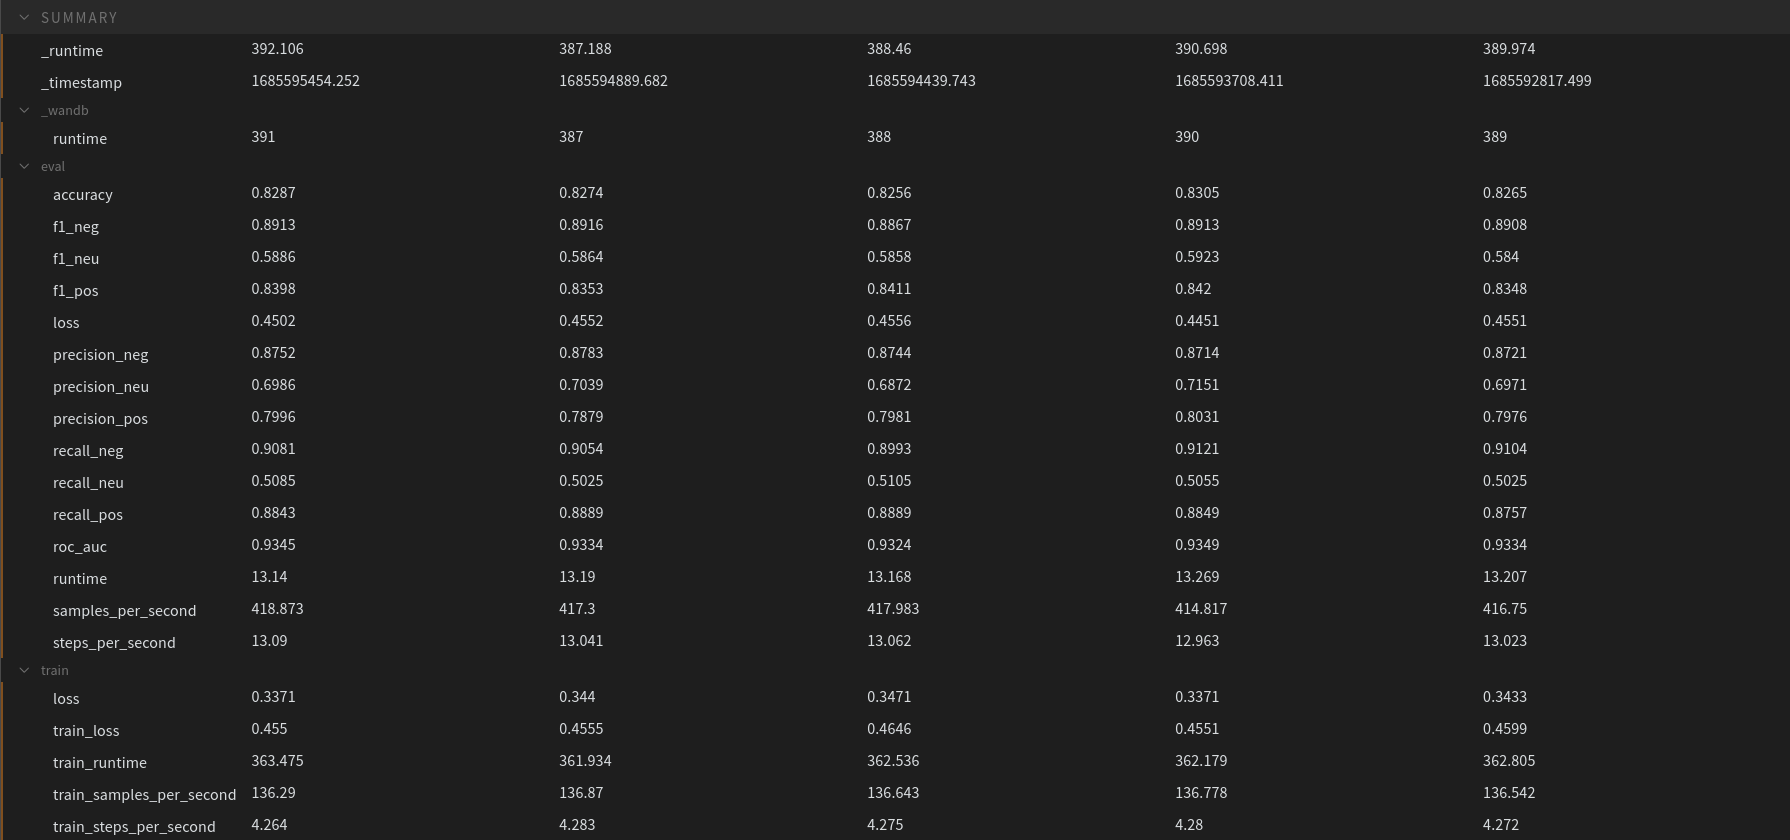
\includegraphics[width=\textwidth,height=6.5cm]{images/baseline.png}
	\caption{Baseline model performance\cite{wandb}}
	\label{fig:baseline}
\end{figure}
\begin{figure}[h!]
	\centering
	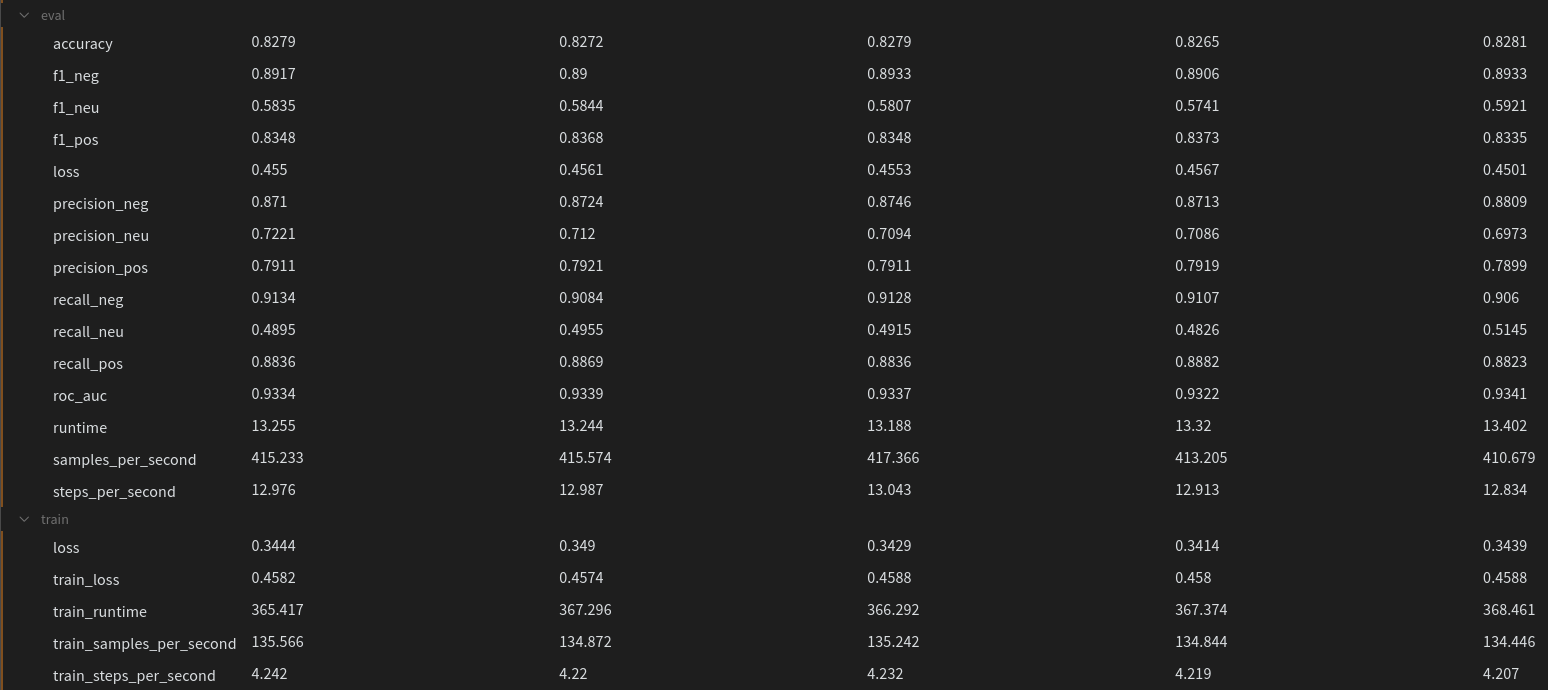
\includegraphics[width=\textwidth,height=6cm]{images/ACARIS.png}
	\caption{ACARIS model performance\cite{wandb}}
	\label{fig:ACARIS}
\end{figure}

\section{Validation}
To validate our approach, we compare the performance of our model to the performance of a baseline model. We use the same model, DistilBERT, but without user embeddings $e_u$. We fine-tune both models on the same dataset and compare their performance on the same test set.\\\\
The base model performed as follows:
\begin{lstlisting}
	Baseline metrics:
              precision    recall  f1-score   support

         neg       0.88      0.90      0.89      1514
         neu       0.63      0.47      0.54       461
         pos       0.81      0.89      0.85       778

    accuracy                           0.83      2753
   macro avg       0.77      0.75      0.76      2753
weighted avg       0.82      0.83      0.82      2753

[[1369   85   60]
 [ 146  217   98]
 [  45   44  689]]
ROC AUC: 0.9355478295192009
Log loss: 0.43026491940343037
\end{lstlisting}
The ACARIS model performed as follows:
\begin{lstlisting}
	ACARIS metrics:
              precision    recall  f1-score   support

         neg       0.89      0.90      0.89      1514
         neu       0.62      0.50      0.55       461
         pos       0.81      0.88      0.85       778

    accuracy                           0.83      2753
   macro avg       0.77      0.76      0.77      2753
weighted avg       0.82      0.83      0.82      2753

[[1361   90   63]
 [ 134  232   95]
 [  36   54  688]]
ROC AUC: 0.9343263777788224
Log loss: 0.43922137166238784
\end{lstlisting}
\break
\section{Results}
\begin{figure}[h!]
	\centering
	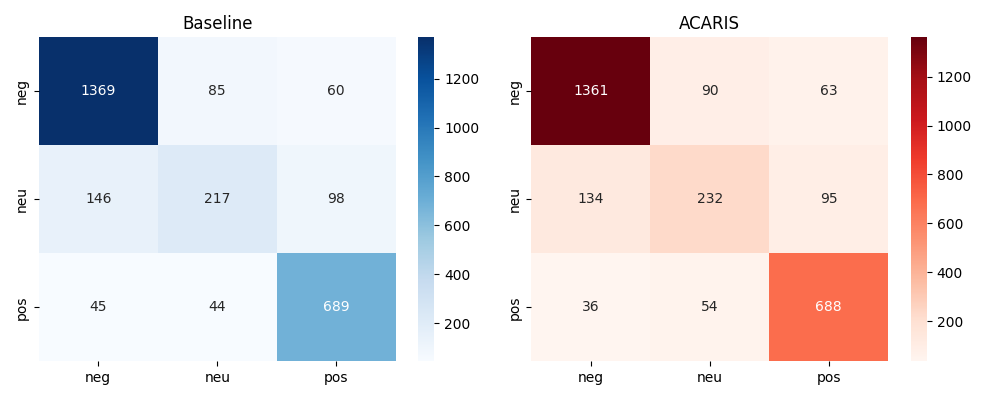
\includegraphics[width=\textwidth,height=6cm]{images/confusion_matrix.png}
	\caption{The confusion matrix of both models}
	\label{fig:Conf}
\end{figure}
Both models performed similarly.

\section{Conclusion}
Given all the information and performance metrics presently available as a result of the current implementation, we must conclude that we failed to reject the null hypothesis $H_0$, and as such, in this particular work, rejected the hypothesis $H_1$. The ACARIS model does not exhibit any statistically nor practically significant improvements over the baseline model.

\section{Future work}
Generally speaking, we still believe that the first part of the hypothesis $H_1$ applies, and that individualizing model outputs to each user is the way to go. It's just a matter of data sufficiency and correct approach. We plan to continue experimenting with various pre-trained models, especially those released in the recent weeks, such as the Falcon-40B\cite{falcon40b}, which performs incredibly well on eval tests, such as the ARC (25-shot)\cite{clark2018think}, HellaSwag (10-shot)\cite{zellers2019hellaswag}, and MMLU (5-shot)\cite{hendrycks2021measuring}, and is presently the number one open-source model\cite{open-llm-leaderboard} in terms of its performance. The recent weeks have also seen numerous optimization techniques that enable more efficient training of larger language models, so even with our limited hardware, we are able to fine-tune models of 13B and more parameters. In addition, we also want to rethink our approach to user embeddings, and perhaps learn them during training, if we find a way to do so efficiently. Until then, we'll continue working with pre-computed user embeddings, but will expand them to add more complexity. Another area of improvement, in our opinion, is the concatenation operation. We believe that summation with word embeddings instead of concatenation may offer different results, and will try to implement it in the future. Finally, and this is the most important factor, is the lack of user-specific data. We don't presently have sufficient messages for many users to train a model that generalizes well, most likely due to our aggressive filtering procedure (all users with less than 25 messages and messages of less than 25 characters are discarded). We suspect that this is the main reason why our model failed to outperform the baseline model.
\newpage

\printbibliography
%\end{multicols}
\end{document}